
\documentclass[thmcnt=section, color=blue, 12pt]{my-elegantbook}

% Index page
\usepackage{imakeidx}
\makeindex[columns=2, intoc, options=-s index_style.ist]

% Title and author
\title{Mathematical Analysis}
\author{Isaac FEI}

% Reference file
\addbibresource{mathematical-analysis.bib} 

% Image of the book cover
\cover{cover}

\begin{document}

% Print title and cover page
\maketitle

%--------
% Preface
%--------

\frontmatter
\chapter*{Preface}

This book mainly follows the structure of \cite{apostolMathematicalAnalysisModern1974}.

%------------------------------

% Print table of contents
\tableofcontents
\mainmatter

%-------------------------------
% Main document starts from here
%-------------------------------

%==============================

\chapter{Point-Set Topology}

%==============================

\chapter{Functions of Bounded Variation and Rectifiable Curves}

%------------------------------ 

\section{Functions of Bounded Variation}

\begin{definition}
	Let $[a, b]$ be an interval.
	A set of points
	\begin{align*}
		P = \{ x_0, x_1, \dots, x_n \}
	\end{align*}
	satisfying
	\begin{align*}
		a = x_0 < x_1 < \cdots < x_n = b
	\end{align*}
	is called a \textbf{partition}\index{partition of an interval} of $[a, b]$.

	The interval $[x_{k-1}, x_k]$ is called the $k$-th subinterval of $P$,
	and we oftern write $\Delta x_k = x_k - x_{k-1}$.

	The collection of all partitions of $[a, b]$ is denoted by $\PC [a, b]$.
\end{definition}


\begin{note}
	In mathematics texts, we have another definition of partitions,
	which states that a partition of a set $S$ is a collection of subsets of $S$
	such that they are disjoint and their union equals $S$.
	We should not confuse these two definitions.
\end{note}

\begin{definition}
	Let $f$ be a real-valued function on $[a, b]$.
	If $P = \{x_0, \dots x_n\}$ is a partition of $[a, b]$,
	write $\Delta f_k = f(x_k) - f(x_{k-1})$.
	If there exists a positive number $M$ such that
	\begin{align}
		\sum_{k=1}^n \abs{\Delta f_k} \leq M \label{eq:1}
	\end{align}
	for all partitions $P$ of $[a, b]$, then we say that $f$
	is \textbf{of bounded variation}\index{functions of bounded variation}
	on $[a, b]$.
\end{definition}

A simple observation is that a function of bounded variation is also bounded.

\begin{proposition}
	Let $f$ be a function of bounded variation on $[a, b]$.
	Then $f$ is bounded on $[a, b]$.
\end{proposition}

\begin{proof}
	By definition, there exists $M > 0$ such that \eqref{eq:1} holds
	for any partitions of $[a, b]$.
	For any $x \in (a, b)$, consider the partition $P = \{a, x, b\}$.
	We have
	\begin{align*}
		\abs{f(x) - f(a)} + \abs{f(b) - f(x)} \leq M
	\end{align*}
	This implies that $\abs{f(x) - f(a)} \leq M$, which further
	implies $\abs{f(x)} \leq \abs{f(a)} + M$.
	Note that $x$ is arbitrarily chosen from $(a, b)$.
	Therefore, $f$ is indeed bounded on $[a, b]$.
\end{proof}

But a bounded function is not necessarily of bounded variation.

\begin{example}
	Consider the function
	\begin{align*}
		f(x) = \begin{cases}
			       \cos \frac{1}{x}, & x \in (0, 1] \\
			       0,                & x = 0
		       \end{cases}
	\end{align*}
	Its graph is shown in Figure~\ref{fig:1}.
	\begin{figure}[H]
		\centering
		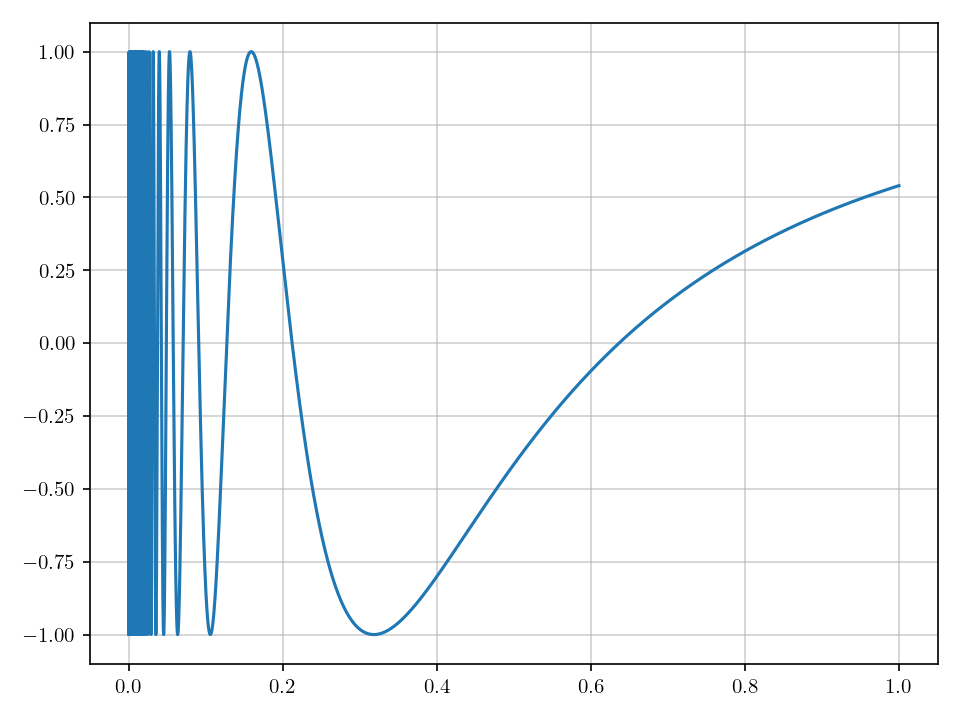
\includegraphics[width=0.6\textwidth]{figures/bounded-function-that-is-not-of-bounded-variation.png}
		\caption{Graph of the function $f(x) = \cos(1/x)$, $x \in (0, 1]$ and $f(0) = 0$. It is bounded on $[0, 1]$ but not of bounded variation for it varias rapidly near $x=0$.}
		\label{fig:1}
	\end{figure}
	Clearly, this function is bounded by $1$.
	But intuitively, it is not of bounded variation since it varies rapidly
	near $x=0$.
	Let $P$ be a partition of $[0, 1]$ where each $x_k$ is given by
	\begin{align*}
		x_k = \begin{cases}
			      \frac{1}{(n-k) \pi}, & 1 \leq k \leq n-1 \\
			      0,                   & k = 0             \\
			      1,                   & k = n
		      \end{cases}
	\end{align*}
	For $k=1, \dots, n-1$, we have
	\begin{align*}
		f(x_k) = \cos ( (n-k) \pi ) \in \{-1, 1\}
	\end{align*}
	The function value is either $1$ or $-1$ and the sign alternates between
	each two consecutive points. Hence,
	\begin{align*}
		\sum_{k=1}^{n} \abs{\Delta f_k}
		\geq \sum_{k=2}^{n-1} \abs{\Delta f_k} = 2 (n - 2)
	\end{align*}
	As we increase the number of points in the partition, $\sum \abs{\Delta f_k}$
	will exceeds any given number.
	Therefore, $f$ is not of bounded variation on $[0, 1]$.
\end{example}



%==============================

% References
\printbibliography[heading=bibintoc, title=References]

%==============================

% Print index page
\printindex

\end{document}
